\documentclass[a4paper,11pt]{article}
\usepackage{graphicx}
\usepackage{natbib}
\usepackage{amsmath}
\usepackage[margin=1.5in]{geometry}
\bibpunct{[}{]}{;}{a}{}{,} 
\bibliographystyle{named}
\begin{document}
\title{Detecting leukaemia from blood samples using Convolutional Neural Networks}
\author{Mbongeni Marketso \n}
\date{\today}


\begin{titlepage}
    \begin{center}
        \vspace*{1cm}
            
        \Huge
        \textbf{Detecting Leukaemia from blood samples using Convolutional Neural Networks}
            
        \vspace{1.5cm}
        \LARGE
        Research Proposal
            
            
        \textbf{Mbongeni Maiketso}\\
        \textbf{306825}\\
  
        \LARGE
        \vspace{1.0cm}
        Supervised by\\
        \textbf{Dr Pravesh Ranchod}    
        \vfill
            
        A proposal presented for the masters degree in\\
        Computer Science
            
        \vspace{0.8cm}
            
        
\includegraphics[width=0.4\textwidth]{WitsUniversitylogo.jpg}
            
        \Large
        Computer science and applied mathematics\\
        University of the Witwatersrand\\
        South Africa\\
        \date{\today}
            
    \end{center}
\end{titlepage}


\begin{abstract}
 In South Africa, there is a shortage specialists that have the necessary expertise to diagnose leukaemia. As a result, blood samples require transportation to centralized referral centres, increasing the turn around time and the risk to patient's lives. Leukaemia can be either acute or chronic. Acute leukaemia develops rapidly hence, the process of diagnosis must be nimble in order to commence with treatment as quickly as possible. In addition, early detection increases the chances of the effectiveness of the treatment. The problem is two fold, we need to reduce  the amount of time it takes for a patient to get diagnosed and we need to make the test accessible. Machine learning has been showing promising performance in image recognition tasks. In particular the use of convolution neural networks has been shown to perform well in image classification tasks. To solve the above mentioned problem we propose building a system that reduces the time it takes for a patient go get diagnosed. The system will receive as input an image of the blood sample, the image will be passed through a convolution neural network and return as output, an indication of whether there are markers that indicate the presence of a leukaemia. To use the haematologist effectively we need to screen the blood samples quickly using the system and prioritise them before they get to the haematologist for diagnosis. 
\end{abstract}
\newpage

\tableofcontents

\newpage

\section{Introduction}
Many breakthroughs have recently been made in the study of artificial intelligence, specifically in the field of machine learning. Machine learning is an umbrella term which encompasses supervised learning, unsupervised learning and reinforcement learning.  This research is particularly interested in supervised learning which is defined by the method in which computer learning occurs. An Algorithm is given a training dataset for which the correct output is known, allowing the algorithm to construct a mapping that can operate on unseen data. Application of neural networks will be investigated in the field of medicine, in particular within the subspeciality of haematology to aid  with the rapid diagnosis of Acute Leukaemia. 

Acute Leukaemia is a cancer of the blood which is fatal if left untreated, however if detected early can be cured \citep{Greaves}. As such, the speed of diagnosis is crucial to the treatment process.The process of diagnosing leukaemia is as follows; Blood samples are taken from the patient and placed in a slide. The slide is taken to a haematologist to determine if the blood sample contains cancerous cells. To do this the haematologist examines the blood sample under a microscope looking for particular visual markers that indicate the presence of a leukaemia. The results are recorded and sent back to the hospital at which point prognosis can begin. The process has a turnaround time of approximately a week or more depending on the patient's proximity to the haematologist. In most cases this delay can be the cause of death for the patient.

Application of machine learning techniques, particularly image recognition can help expedite this process. Diagnosis of acute leukaemia by a haematologist requires macroscopic analysis of blood samples under a compound light microscope. As part of the outcome of this research we intend to build a tool that can aid diagnosis. In essence we want to build a system that can analyse blood samples and provide a screening tool to detect an acute leukaemia. In
this research, we will be performing a replication study of \cite{Sara}, with the aim of verifying the results but more importantly to produce a system that can be used to aid diagnosis.

The rest of this document is structured as follows: In section \ref{background} we give a biomedical background of leukaemia to aid the reader with regards to the medical problem. In section \ref{machineLearning}, we discuss machine learning in detail followed by a brief history of machine learning in section \ref{relatedWork} where we look at the related work and what other researchers have done. Concluding remarks are provided in section \ref{conclusion}.
\section{Background and related work}
\label{background}
\subsection{Introduction}
In this section we briefly discuss what leukaemia is and also show why we believe that machine learning techniques can be used to  aid the diagnosis of leukaemia. We discuss leukaemia with the intention to provide the reader with enough background to understand why it is possible to use machine learning to detect leukaemia in blood samples. In section 2.3 we discuss machine learning and the different approaches, such as supervised learning and unsupervised learning. A discussion about artificial neural networks and deep learning, the core theme of this research comes next. Following the discussion on deep learning we take a deep dive into convolution neural networks,  why they are powerful in machine learning particularly in image recognition and classification tasks. At this point we would have built a foundation of the tools available from machine learning and also explained why the diagnosis of leukaemia can be aided by the use of such tools. In section 2.5 we will survey the literature for related work on using machine learning techniques to help diagnose diseases, specifically diagnosing leukaemia. Here we will see that there has been exceptional results achieved in the accuracy of the models built to diagnose leukaemia and other disease where diagnosis is done by examination of blood samples through a microscope. Section 2.6 provides a conclusion.
\subsection{Biological and medical background of leukaemia}
\label{section: medical}
Leukaemia is a life-threatening haematological malignancy that is characterized by an uncontrolled
proliferation of the body's white blood cells namely monocytes, eosinophil, lymphocytes, basophils and neurophils. The malignant clone originates in the bone marrow and will generally spill out into the peripheral blood. Leukaemia can be classified as either acute or chronic. For the purposes of this research, only acute leukaemia will be discussed as this entity is a more life-threatening condition compared to chronic leukaemia. In addition, the subclassification goes on to further define the specific lineage of the leukaemia, that is, whether it belongs to the lymphoid or myeloid lineage, Acute Lymphoblastic Leukaemia (ALL) and Acute Myeloid Leukaemia (AML) respectively \citep{Jakkrich}. 

To understand what leukaemia is we need to understand the normal life cycle and function of white blood cells. Leukaemia is fundamentally a maturation arrest at the primitive stage of the cell's normal life cycle. Blood cells are made in the bone marrow; the soft tissue located inside the inner cavity of certain bones\citep{Janeway}. Bone marrow is predominantly comprised of haemopoietic cells which give rise to all the blood cells of the body namely red blood cells, white blood cells and platelets. Stem cells have 2 unique abilities: to identically replicate themselves and to differentiate. The term differentiate explains the process of a cell maturing and becoming a different blood cell from the its predecessor, a so called ‘daughter’ cell. Stem cell can be thought of as an infant, with unlimited potential to become anything he/she wants, in this case the stem cell has the ability to become any of the cells found in the blood: red blood cells, white blood cells, platelets etc \cite{blood}. 

When stem cells differentiate, they mature into either common myeloid progenitor cells or lymphoid progenitor
cells, the first recognizable separation of lineage committed progenitors. For the sake of simplicity, these can be thought of as the young child growing up and choosing certain school subjects that will enable/limit specific career paths. In other words, the differentiation of common myeloid progenitor cells will restrict their lineage potential and will only go on to ever produce specific type of blood cells, including red blood cells, neutrophils and monocytes etc, but never others such as
lymphocytes. Likewise, the lymphoid progenitor cells are forever constrained to produce only
lymphocytes: specifically the T and B lymphocytes, as seen in Figure \ref{fig: stemCells1}. The common myeloid progenitor cells will further differentiate and eventually give rise to myeloblasts, the earliest recognizable myeloid precursors and so too will lymphoid progenitor cells differentiate to become lymphoblasts, the earliest recognizable lymphoid precursors \citep{Janeway}.

 \begin{figure}[!htbp]
 \begin{center}
  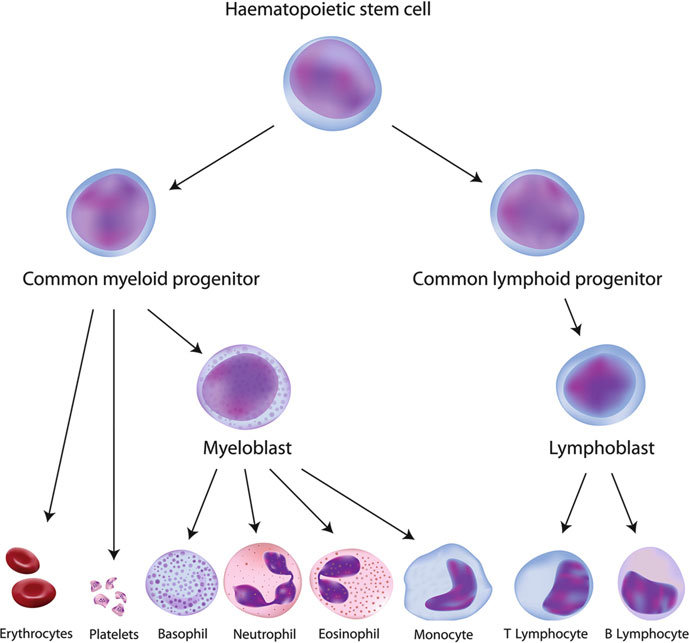
\includegraphics[scale=0.4]{WhiteBloodCell.png} 
  \end{center}
  \caption{White blood cell evolution \citep{phdthesis}}
  \label{fig: stemCells1}
 \end{figure}

This is analogous to the young adult graduating from a final career choice. 
The myeloblasts and lymphoblasts will differentiate into the actual mature white blood cells, able to perform their respective functions. The function of white blood cells is ultimately to fight infections. Lymphocytes, constitute part of the adaptive immune system, and protect the body from invading germs by developing into plasma cells, which produce antibodies. The antibodies attach and coat the germs (bacteria, viruses, and fungi), which helps other white blood cells (the macrophage) recognize and destroy them. acute lymphoblastic leukaemia is a condition in which the lymphoblasts (immature cells) divide uncontrollably and spread throughout the bone marrow rapidly. Since lymphoblast are immature cells, they are not able to perform the normal functions of their mature counterparts and are unable to adequately fight infections. In addition, because these cells proliferate so fast, they invade the space for normal haemopoietic cells resulting in the body not being able to produce normal blood cells. Now that we have a basic understanding of the pathophysiology of acute leukaemia, let us discuss the process of diagnosis in order to explain why machine learning techniques can help automate this
process. Numerous possible diagnostic methods, including peripheral blood smear review, bone
marrow aspirate and trephine biopsy, lymph node biopsy and flow cytometry analysis, can facilitate the diagnosis of an acute leukaemia. The most economic approach is to examine microscopic images of peripheral blood samples using the compound light microscope. A haematologist will examine the patients peripheral blood sample, spread and stained on a glass slide, and manually count the number of blasts (immature blood cells) present. A cut off threshold of 20 percent of blast cells relative to all the cells on the slide is in keeping with a diagnosis of acute leukaemia. The manual count is a labour-intensive task and prone to error. Figure \ref{fig: compare} shows a comparison of normal (Healthy) lymphocyte morphology compared to morphological features of blasts. Machine learning provides techniques for classifying images by learning patterns from large datasets. In the following section we discuss machine learning and why it is well suited to solve this problem.

 \begin{figure}[!htbp]
 \centering
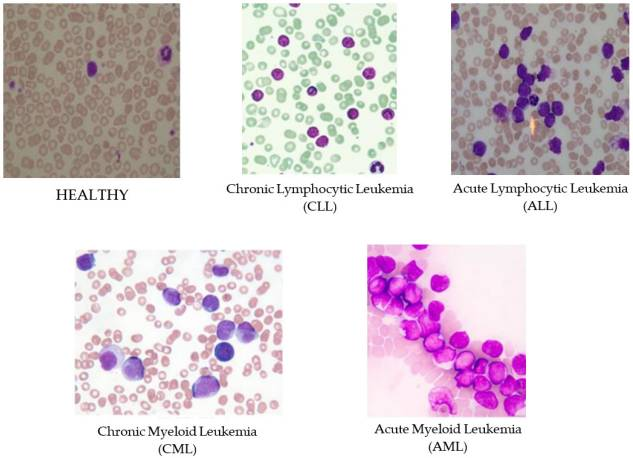
\includegraphics[scale=0.5]{ImDB2.jpeg} 
  \caption{Blasts vs Lymphocytes \citep{Ahmed}}
  \label{fig: compare}
 \end{figure} 
 
\subsection{Machine learning}
\label{machineLearning}
In this section we refer to \cite{Stephen}, unless otherwise specified. Machine learning is sub-field of artificial intelligence which is concerned with developing algorithms that extract pattens (learn functions) from a dataset. Machine learning is divided into different branches based on the learning approach, below we give a brief description of each.

\paragraph{Unsupervised learning:}
In unsupervised learning, correct answers are not provided, however the algorithm learns common features in the data and uses these features to group or categorise the inputs together.

\paragraph{Supervised learning:}
Supervised learning is the category that houses most machine learning algorithms(i.e, the most widespread technique). In supervised learning, the algorithm gets told what the correct answer is. The intention of the algorithms is  to learn from data using the correct answer as guidance to get to a general solution. The general solution can then be applied to data  that has not been seen. As part of the training, the algorithm is told how to move to the correct answer. 

\paragraph{Reinforcement learning:}
In reinforcement learning, algorithms are commonly referred to as an agents,  the learning agent takes actions so as to maximise a reward. The agent is presented with a situation in which there are multiple possible actions to take, each action has an associated reward. The agent tries out these actions with the purpose of maximizing the reward \citep{Sutton1998}. 

\paragraph{}
In the opening statement of this sections we said that machine learning is a subfield of artificial intelligence which is concerned with developing algorithms that extract pattens (learn functions) from a dataset.  There are three ideas here that are worth elaborating on. Namely the idea of learning, the idea of a function and the dataset. Datasets can be represented in different ways. For example a table with rows and columns could represent a dataset where each row represents an instance of the dataset. A dataset of images can be represented using matrices were each matrix represents an image and each entry in the matrix represents a pixel.

The second idea that we need to discuss is learning. In this context, learning refers to the process of extracting patterns from a dataset, patterns are referred to as functions or models. In essence we are looking for a function that represents patterns in the dataset. A function is a deterministic mapping of inputs to outputs \citep{John}. That is, given an input, a function will always produce the same output. To give an example consider the dataset in table \ref{tab: datasetExample}. 

\begin{table}[!htbp]
\begin{centering}
\begin{tabular}{|c|c|c|}

\hline 
Salary (R) & Debt payment(R) & Credit score \\ 
\hline 
15000 & 10000 & 100 \\ 
\hline 
25000 & 30000 & -50 \\ 
\hline 
45000 & 25000 & 400 \\ 
\hline 
20000 & 35000 & -300 \\ 
\hline
\end{tabular} 
\caption{Example of simple dataset}
\label{tab: datasetExample} 
\end{centering}
\end{table}


The table has three columns; monthly salary, monthly debt repayments and credit score. A machine learning algorithm can be used to learn a pattern or function that relates a person's income and debt payment to their credit score. In image classification, we could have a dataset of images represented by matrices and a machine learning algorithm can be used to learn patterns in the images. The patterns are used to build models.  In a nutshell, to understand what machine learning is, we need to understand three phrases. Dataset, algorithm and function. An algorithm describes the process we use to learn, a function is a pattern that models the dataset(sometimes referred to as the model). The dataset is our domain or the search space, in our case the set of images containing blood sample and cells. There are many ways to represent functions.  Machine learning functions are represented using artificial neural networks.  In the next section we will briefly discuss what artificial neural networks are and how they are used to represent functions.

\subsubsection{Artificial neural networks}
\label{section: ANN}
The use of artificial neural networks draws inspiration from biology, more specifically from how the brain works. In animals, learning happens in the brain. The brain is made up of nerves called neurons. Each neuron is connected to other neurons to form a network. Neurons are basic working units of the brain, they transmit information to each other in the form of electrical signals also known as impulse. Figure \ref{fig: neuron} shows a picture of a basic neuron.

 \begin{figure}[!htbp]
  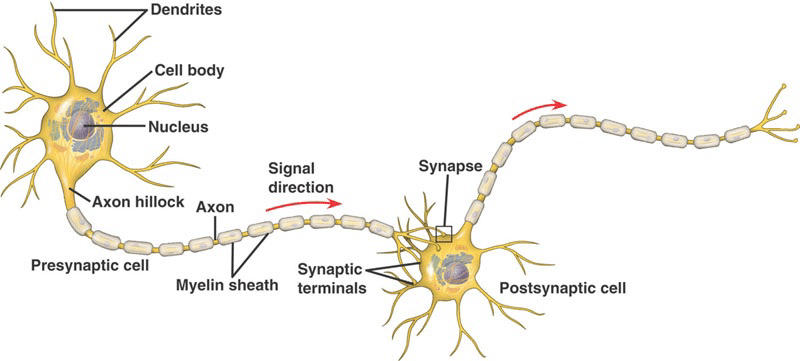
\includegraphics[scale=0.5]{neuron-structure.png} 
  \caption{Picture of a basic neuron \citep{Grau}}
  \label{fig: neuron}
 \end{figure}

 The artificial neuron, the perceptron works in a similar fashion. It computes a weighted sum of inputs. A activation function determines whether the perceptron is activated or not.  Figure \ref{fig: perceptron} shows an image of a perceptron. Mathematically, a perceptron can be represented as follows:
 
 \begin{equation}
  h = \sum_{i=1}^{n} w_ix_i
 \end{equation}

Where h represents the weighted sum of the inputs on a neuron. 
 The inputs and weights are represented by the $x_i, w_i$ respectively. A simple activation function can be written as below:
 
 \begin{equation}
    g(h)=
    \begin{cases}
      1, & \text{if}\ h > 0 \\
      0, & \text{if}\  h \le 0
    \end{cases}
  \end{equation}

\begin{figure}[!htbp]
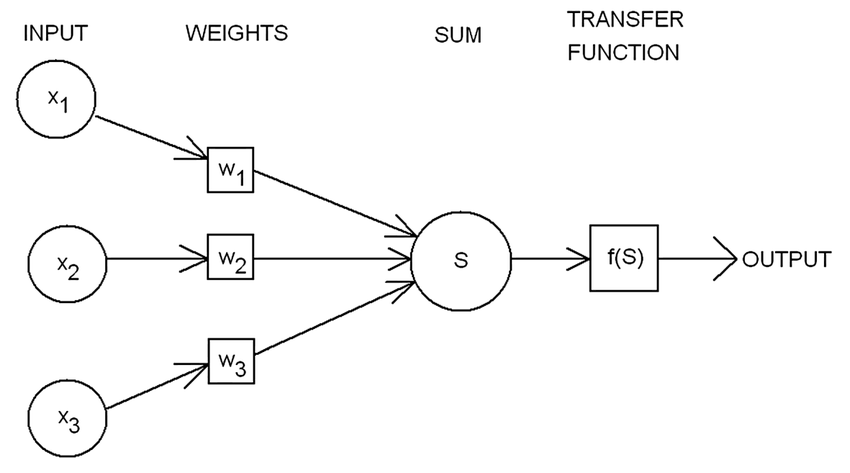
\includegraphics[scale=0.5]{Perceptron_1.png}  
\caption{Picture of a single perceptron \citep{Alves} }
\label{fig: perceptron}
\end{figure}
 
In machine learning we use artificial neural networks to represent functions. Each neuron receives input, computes the weighted sum of the inputs and feeds the weighted sum to an activation function. The output of the activation function can be used as a classifier. In order to accurately classify the input, the correct set of weights need to be learned. The process of learning can be thought of as the process of searching for weights for each edge of an artificial neural network. In their simplest, form artificial neural networks have an input layer and an output layer. The input layer is used to take in the input and the output layer produces the output. 

In order to learn complex functions more layers are inserted into the network to create a neural network with an input layer, an output layer and one or more hidden layer(s). An artificial neural network that has one or more hidden layer(s) is called a deep neural network. Figure \ref{fig: ANN}, illustrates an artificial neural network with two hidden layers. In the following section we briefly describe deep neural networks and deep learning.

 \begin{figure}[!htbp]
  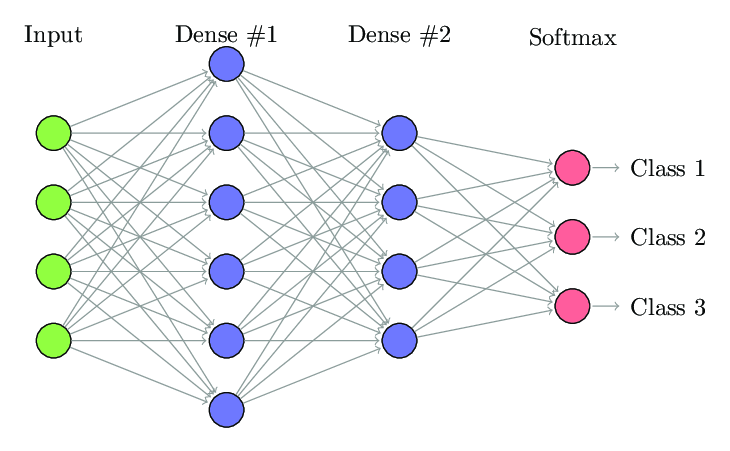
\includegraphics[scale=0.5]{ANN.png} 
  \caption{Picture of an artificial neural network \citep{Pelletier} }
  \label{fig: ANN} 
 \end{figure}

\subsubsection{Deep learning}
\label{deepLearning}
The phrase deep learning is coined from the use of artificial neural networks that have more than one hidden layer also known as deep neural networks. Increasing the number of neurons within a layer and increasing the number of layers has been shown to improve the accuracy of the artificial neural network. As a result, there is a growing body of research on the architecture of artificial neural networks in order to find the best architecture \citep{Alzubaidi}. A neural network  architecture has an impact on the time it takes to train the model, additionally a good architecture improves the accuracy of the model \citep{John}. In section 2.3 we mentioned that in order to understand machine learning we need to understand three components. One of those components is the algorithm, that is, how is a neural network is actually trained. In the following section we introduce an algorithm called gradient descent. The gradient descent algorithm provides a way to update the weights of a artificial neural network such that we improve the prediction accuracy of the network. 

\subsubsection{Gradient descent}
The process of training  artificial neural networks can be characterised by randomly initialising the neural network weights and updating the weights based on how good the network performs against the training data. The weights are updated iteratively until the network performs as expected. The gradient descent algorithm is used to define the learning rule to update the weights. Using $t$ to denote the iteration of the algorithm where an iteration is a single parse of the algorithm through a single item in the dataset, $W$ to denote the weights, $Y$ to the error of the output of the weighted sum the rule to update the weights can be written as follows.

 \[ W_i^{t+1}= W_i^{t} + \left( \eta  \times \sum_{j=1}^{n} \left( \left(Y_j^t -  \sum_{i=1}^{m}w_i \right)\times x_{j,i}  \times x_{j,i}\right) \right) \]

Having defined the weight update rule as above, the gradient descent algorithm can be summarised as follows.

\begin{enumerate}
\item Initialise the model with a random set of weights.
\item Run the model though the dataset until it yields the expected performance.
\subitem a) Apply the current model to the dataset
\subitem b) Adjust the weights using the weight update rule
\item Return the final model with the optimised weights.
\end{enumerate}

Since the gradient descent algorithm updates the weights of a single neuron, for neural networks containing multiple layers the update rule suffers the credit assignment problem. That is which neurons are responsible for what portion of the error. To solve this problem the backpropagation technique is used.

\subsubsection{Backpropagation}
\label{backprop}
For this section we refer to \cite{John}. The backprogation algorithm is an algorithm used to update the weights of a neural network. The backpropagation algorithm begins by randomly initialising the weights of the   neural network. Once the weights are initialised the network can be trained by first presenting it with the input. At each stage for each neuron we keep track of the weighted sum and the value of the output of the activation function respectively. The aim is to iteratively update the weights of the network until the network reaches an acceptable level of performance. The second step of the algorithms is to calculate the error gradient of each neuron in the output layer.  We also calculate the error gradient of the network with respect to changes in the weights of the network. These are the gradients that  we use to update the weights of the network.


\subsubsection{Convolution neural networks}
\label{convolution}
Convolution neural networks(CNN) were originally designed for image recognition tasks but they can be used for other tasks such a speech recognition \citep{John}. In section \ref{section: ANN} we described artificial neural networks, we mentioned that each neuron learns a small portion of the function being modelled and combining all the neurons in the network gives a complex function being modelled. With convolution neural networks the idea is the same however, convolution neural networks have been designed so that the earlier  neurons learn low level visual features and the later neurons combine these features to learn high level features. In addition, the idea with CNNs is to preserve the spatial information of the pixels in the image \citep{John}. In this section we describe how CNNs work and we refer to \cite{Ian}. CNNs have different types of layers; the convolution layers, pooling layer and output layer, see Figure \ref{fig: convOp}. In the convolution layer we slide a filter along the input, do an element wise multiplication and sum the products to get a scalar value. With CNNs not every node is connected to every other node in the next layer as in fully connected neural networks, this reduces overfitting as there are less parameters to learn. The second layer of a CNN is the activation layer. In the activation layer typically the leakey reLu or softmax is used to determine whether a neuron is active or not. Subsequent to the activation layer, is the pooling layer. Pooling is for downsampling of features so that less parameters are learned during training. There are two hyperparameters that control this, the dimension of spatial extent, that is the dimension of what we are looking to extract a feature and the stride. The stride is the step that the filter moves along the input. In practice normally max pooling is used, that is, we take the maximum value in the input channel. The first three layers are sometimes referred to collectively as the convolution layer, the next layer is the fully connected layer, identical to fully connected layer in a traditional neural network.  One of the challenges of designing an architecture of a neural network for image recognition is that the design must be such that the network will be able to detect the feature anywhere in the image. For example if we are looking for a picture of an abnormal cell, the network should be able to identify the abnormal cells irrespective of its location in the image. Convolution neural networks have been designed to deal with this challenge as \cite{Yann} stated in paper titled Generalization and Network Design Strategies . To explain this we have to look at where convolution neural networks get their name from. CNNs get their name from the fact that they follow a sequential process for searching through an imgage for features by applying the same function at each region for each layer, this process is called convolving \citep{John}. Most CNNs employ a three step approach. 1) The first step is to apply convolution across the entire image, then apply a non-linearity and finally down sampling  by using a down-sampling function. 

\begin{figure}[!htbp]
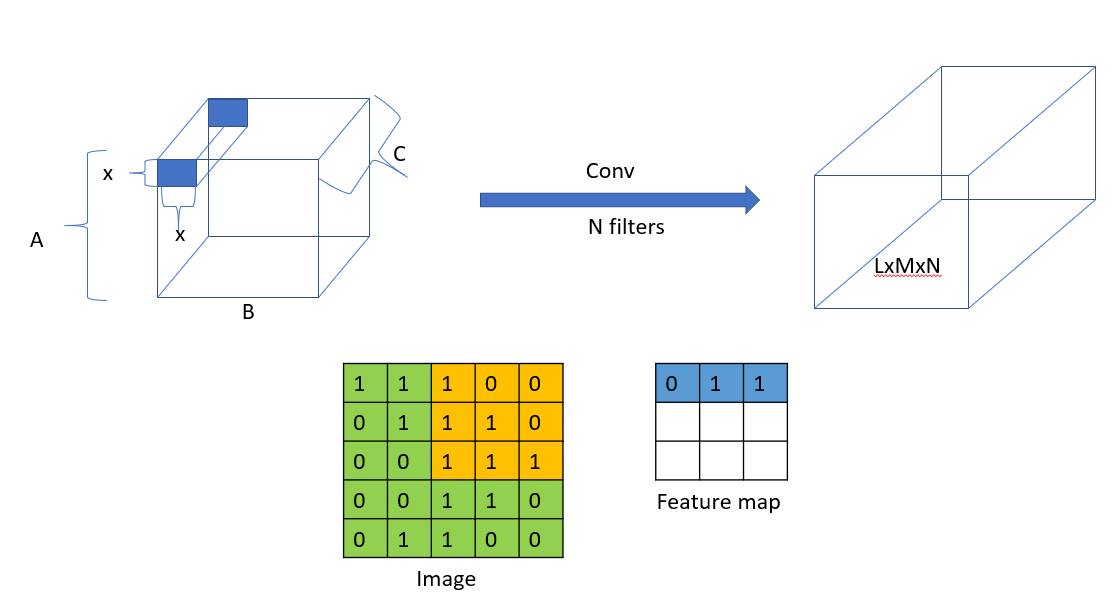
\includegraphics[scale=0.5]{ConvolutionOperation.jpg} 
\caption{Picture of the convolution operation}
\label{fig: convOp}
\end{figure}
The ImageNet dataset consists of thousands of images. The aim is enabling researchers to evaluate algorithms for object detection and image classification. There is a challenge where each year researchers submit algorithms where the objective is to identify the best algorithm for object detection and image classification. In the following section we discuss various architectures and their performance on the ImageNet challenge. 

\subsection{History of convolution neural networks}
\cite{AlexNet} produced ground breaking research in computer vision, specifically image classification. A convolution neural network with 60 million parameters and 650 000 neurons was built. The architecture of the CNN consists of five convolution layers. Some of the convolution layers where interspersed with some max-pooling layers followed by fully connected layers and an output layer made up of a softmax layer of 1000 neurons \citep{AlexNet}. Figure \ref{fig: AlexNet} shows the architecture of the CNN. Alexnet achieved a performance error rate of 36.7\% in the ImageNet challenge. 

\begin{figure}[!htbp]
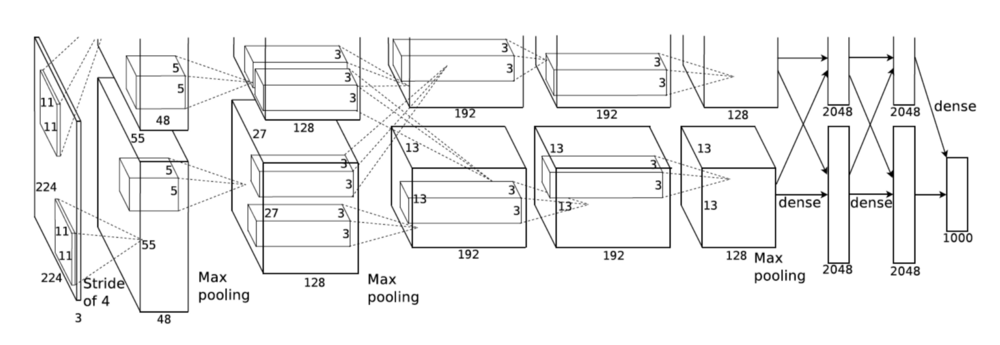
\includegraphics[scale=0.3]{AlexNetArchitecture.png} 
\caption{Architecture of AlexNet CNN \citep{NIPS2012_c399862d} }
\label{fig: AlexNet}
\end{figure}

With AlexNet having paved the way for CNNs in computer version,  \cite{ZFNET} improved on the performance of AlexNet, achieving an error rate of 11.2\% on the ImageNet dataset. The main improvement over AlexNet from an architecture perspective is the use of a 7x7 filter instead of a 11x11 filter used in Alexnet in addition a smaller stride was used this retains more pixel information compared to AlexNet \citep{ZFNET}. Further improvements by \cite{simonyan2015deep} were achieved, reaching an error rate of 7,3\%. To achieve these results CNN with 16-19 (VGG-16 and VGG-19) hidden layers was implemented \citep{simonyan2015deep}. Since then, improvements have been achieved by increasing the depth of the CNN with \cite{googleNet} taking the depth to 22 and achieving an error rate of 6.7\% (GoogleNet) and Microsft's ResNet taking it even further with a depths of 152 layers and achieving an error rate of 3.6\% \citep{microsoft}.

In the following section we discuss applications of some of the CNN architectures to medicine.

\subsection{Related work}
\label{relatedWork}
As we have mentioned in previous sections, diagnosis of leukaemia can be done by examining a specimen of blood to detect blasts that indicate the presence of leukaemia. The cells are small and differences between normal cells and malignant cells can be difficult to detect under a microscope. It takes a trained professional to accurately diagnose leukaemia. Based on this, it would be necessary to research if deep learning techniques, particularly CNNs can be applied to detect features in microscopic images to aid  diagnosis of leukaemia. \cite{Ayse} applied deep learning to build a system that automatically detects nano particles in microscopic images. \cite{Ayse} were particularly interested in building a model that would differentiate different types of particles in microscopic images. In the case of blood samples, this would be to recognise malignant cells(blasts) from normal cells. The proposed method used convolution neural network with two outputs, the first output is for identifying the particle and the second output provides the location of the particle in the image. Using this approach \cite{Ayse} achieved accuracy rates of between 96\% and 98\%. Providing evidence that CNNs can be used to detect features in microscopic images of blood samples, however it is important to note that the study was not specifically for detection of leukaemia but for detecting particles in microscopic images. 

The rest of this section discusses different approaches used in previous research projects using CNNs to automatically detect and classify leukaemia in microscopic images of blood samples.

Researchers are using convolution neural networks to build robust computation system that aid in image recognition \citep{Luis}. The use of convolution neural networks for image recognition, more specifically for feature extraction is out performing conventional methods \citep{Luis}. The literature presents two approaches for training convolutional neural networks.

The first approach is  to train the CNN from scratch and the second is to use a technique referred to as transfer learning. With transfer learning, a pre-trained CNN from a different domain is fine tuned for another task. There are  number of challenges that come with training CNNs from scratch. The first being that to train CNNs from scratch requires large amounts of labelled datasets. The second challenge is that training CNNs requires a lot of computing power. In addition training from scratch comes  with problems of overfitting and having to adjust the architecture of the CNN to improve performance  which requires expert knowledge \citep{IEEETransactions}.

An alternative approach especially in the absence of labelled data is to use pre-trained CNNs.
\cite{Luis} used Convolution Neural Networks (CNN) and Support Vector Machines to build a system that diagnosis leukaemia from blood slides. The technique used by \cite{Luis} was to use pre-trained CNNs (AlexNet, VGG-f and CaffeNer) for feature extraction from the images without doing any preprocessing. The extracted features were used for classification with the use of support vector machines(SVM). A hybrid of three datasets. The first dataset consists of blood smears containing one leukocyte, the second dataset contains blood smears with many leukocytes and the third dataset contains a mixture of images with one leukocyte and many leukocytes. A leukocyte  is a type of blood cell that is made in the bone marrow and found in the blood and lymph tissue. Leukocytes are part of the body's immune system. They help the body fight infections and other diseases \citep{Greaves}. Using a hybrid dataset demonstrates the robustness of the approach. Their methodology achieved hit rates above 99\% and outperformed nine methods found in the literature. Feature extraction was done with CNNS and a support vector machine was used to classify the images as pathological or not. It should be mentioned that transfer learning is an approach which is suitable especially when there is a limited amount of labelled data. It would be interesting to know if there is a way to train deep learning models that solve tasks across multiple domains. \cite{Kaiser} researched  this, the architecture they presented had a performance of approximately 86\% on the imageNet dataset.
It has been shown that pushing the CNN depth to 16-19 weight layers can significantly improve the performance of the CNN . It has also been shown that this architecture generalises well to other datasets \citep{simonyan2015deep}. Support vector machines have also been used in the classification of microscopic images of blood samples. In \cite{Nimesh}, a five step approach was used to create a system for automatic detection of leukaemia from blood slides. Firstly images were collected from a hospital and labelled. Secondly images where preprocessed to improve the the quality of the images. Thirdly k-means clustering was applied for detecting white blood cells. When blood samples are placed on slides, cells sometimes stack on top of each other. To detect these cells, a measure of roundness was used. Normal cells that are not stacked on top of each other tend to maintain their roundness. In the final step the features were extracted and classified using support vector machines. The approach achieved 93\% accuracy. 

\subsection{Conclusion}
Section \ref{section: medical} began with a description of what leukaemia is, we discussed the biology of leukaemia with the the  objective to provide the reader with the morphology of the cancer. That is to show how it looks on an image and how a haematologist diagnosis patients. This is important because we are interested in showing that this can be reduced to an image classification problem. We then introduced machine learning using a top down approach, starting from high level concepts such as the different types of machine learning branches in section \ref{machineLearning}. Since our focus is on supervised learning, we elaborated further on supervised learning and tools and techniques used. In section \ref{section: ANN}, we dicussed neural networks  followed by deep learning in section \ref{deepLearning}.  At this point we had demonstrated which machine learning tools we are going to research and why they might work. In section \ref{relatedWork}, we provided a literature survey of the work done by researchers in ascending order of accuracy and finally provided the current state of the art models for image recognition and classification tasks.
\section{Research objectives}
\label{objective}
\subsection{Introduction}
Now that we have discussed what leukaemia is, what machine learning is and the tools available to aid in the diagnosis of leukaemia, we are in a position to introduce our research project. We will state our research objective in section \ref{aim}, followed by the research problem in section \ref{problem}. We will then discuss the motivation for the research project in section \ref{motivation}. Concluding remarks are outlined in section \ref{concludeObjective}.
\subsection{Aim of research}
\label{aim}
The aim of this research is to produce a system to automatically diagnose cancer from pictures of blood samples. The type of cancer in question is Leukaemia, specifically Acute Lymphoblastic Leukaemia (ALL), which as stated earlier in section 2.2 is the most common type of caner among children and it spreads quickly. The system should produce a probability of a blood sample containing ALL given the picture of a blood sample. This probability can then be used to prioritise the attention or urgency to thoroughly diagnose the blood samples. 
\subsection{Research problem}
\label{problem}
The research problem is to identify whether deep learning techniques can be used to identify whether a blood sample contains ALL. In particular we want to know whether having a hybrid architecture for an artificial neural network can provide a level of accuracy that is high enough to use the model in assisting cancer specialist in diagnosing cancer from blood samples. The hybrid architecture will consist of VGG16 and MobileNet. It should be emphasized that this is a replication study of \cite{Sara} 
\subsection{Motivation}
\label{motivation}
In a paper by \cite{Sara}, a hybrid architecture was used to build a model for automatic detection of ALL. The model consists of VGG16 and MobileNet. Figure \ref{fig: vgg16} illustrates the architecture of VGG 16 neural network.  VGG16  consists of 13 convolution layers using 3 x 3 convolution filters followed by max pooling layers and two 4096 fully connected layers followed by a softmax classifier. We refer to \cite{Andrew} to elaborate further on the MobileNet architecture. It is designed to be light weight by reducing the total number of operations while not compromising the performance of the model. In contrast to normal CNN,  MobileNet uses Depthwise seperable convolution which consist of two steps. The first steps, depthwise convolution applies convolution to a single input channel at a time, for instance, if the input is a RGB image with 32x32x3. Depthwise convolution applies convolution to one channel at a time. The second step is pointwise convolution, an application of a 1x1xM filter where M represents the number of input channels(3 in the case of RGB image) is performed.  The architecture by \cite{Sara} consists of depth-wise separable convolution and 11 point-wise convolutions. The results demonstrate that the model yields better prediction than individual models for leukaemia B-lymphoblast classification with 96.17\% overall accuracy, 95.17\% sensitivity and 98.58\% specificity layers. This is a useful level of accuracy and can be applied practically in the real world. In addition, the motivation to produce a system comes from the practical problem that exists in the South African health industry.

Testing for cancer is expensive and only available to those that can afford it. Further more, there is a considerable amount of time from the time a person gets tested to the time they get their results in order to commence treatment. All this delay could be the difference between life and death for some patients hence a system that can help automate or speed up the diagnosis process will have life saving consequences.

\begin{figure}[!htbp]
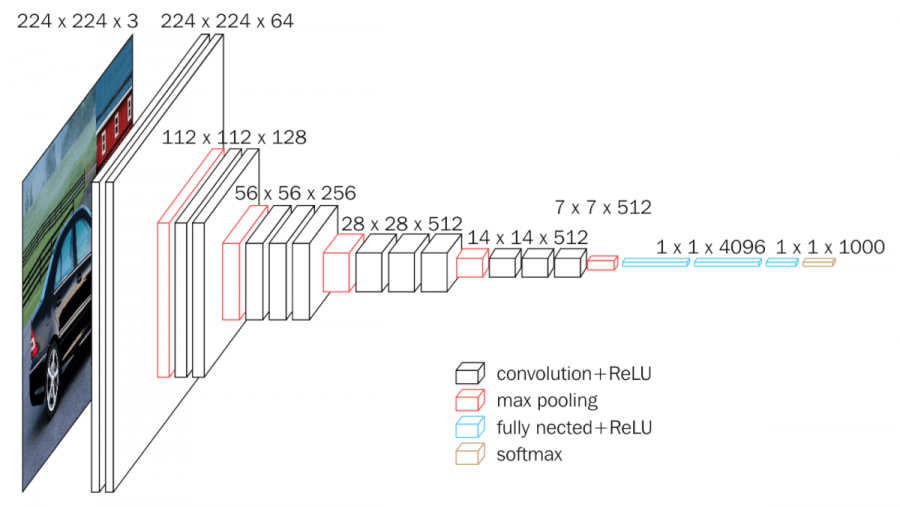
\includegraphics[scale=0.4]{vgg16.png} 
\caption{Picture of the VGG 16 architecture \citep{AlexNet}}
\label{fig: vgg16}
\end{figure}

\subsection{Conclusion}
\label{concludeObjective}
In this chapter we discussed the aim of the research which is to build a system that can automatically provide the probability of a blood sample containing leukaemia cells. This was discussed in section 3.2. In section 3.3 we discussed the research problem. We want to use deep learning techniques to build a model that can automatically detect whether a blood sample has leukaemia or not. The motivation for this research was discussed in section 3.4.  

\section{Research method and plan}
\subsection{Introduction}
In this section we provide a plan for how the research will be carried out. In section \ref{phases} we will give a detailed account of each phase of the project and what we will be doing in that phase. A description of the data set is provided in section \ref{dataset}. We will provide some risks and potential problems that we might encounter in section \ref{risks} and provide a conclusion in \ref{concludeMethod}. 
\subsection{Research phases}
\label{phases}
The research process comprises of six phases. In the first phase we will gather the dataset required to train the model. The dataset will be obtained from the cancer imaging archive made available freely for public consumption. In the second phase, we will use various pre processing techniques, this is to increase the visibility of crucial structures to ensure that the model we train is robust. Training machine learning models requires a huge amount of data, the pre processing stage will result in an increased amount of data which can be used to train the model to make it more robust. The third phase is where we will build the model and the actual training of the model. Using the dataset and the proposed architecture we will train the model. The fourth phase is the testing phase, we will test the model against the testing portion of the dataset. The fifth stage of the research will be to build an actual system that can be used to help in the diagnosis of ALL. In the final phase of the research we will also investigate the performance of the mobile equivalent of the architecture. If the mobile equivalent performs better and produces good results we will build a stand alone mobile application which will be available for download. The system/app will take as input an image and return a probability of the image containing cancerous cells. Figure \ref{fig: timeline} provides a high level of the research project. 
 In the next section we provide a description of the dataset that will be used to train the model.

\begin{figure}[!htbp]
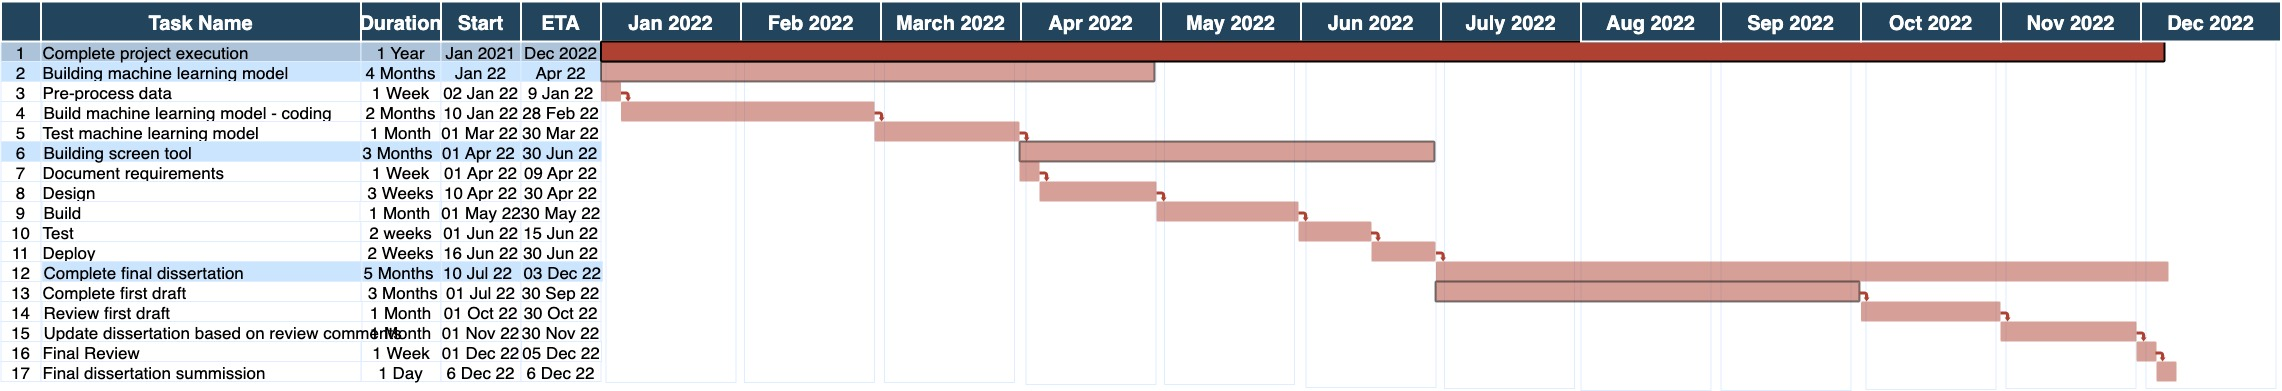
\includegraphics[scale=0.17]{Timeline.jpeg} 
\caption{High level timeline of research project}
\label{fig: timeline}
\end{figure}

\subsubsection{Description of dataset}
\label{dataset}
The dataset constitutes approximately 25\% of paediatric cancers. Total cell images: 10,661, ALL(cancer): 7272, Normal: 3389

\begin{enumerate}
\item Train set:

\begin{itemize}
\item Total subjects: 73
\item ALL (cancer): 47
\item Normal: 26
\end{itemize}


\item Preliminary test set composition: Total cell images: 1867, ALL(cancer): 1219, Normal: 648
\begin{itemize}

\item Total subjects: 28
\item ALL (cancer): 13
\item Normal: 15
\end{itemize}

\item Final test set composition: Total cell images: 2586
\begin{itemize}

\item Total subjects: 17
\item ALL (cancer): 9
\item Normal: 8
\end{itemize}
\end{enumerate}

\subsubsection{Evaluation method}
To evaluate the performance of the model, we will follow the method described by \citep{Sara}. Three metrics will be used, namely accuracy, sensitivity and specificity. Below we provide equations for calculating the above metrics.

\paragraph{}
 Accuracy is measured by taking the ratio of correctly classified images to the total number of test images. Accuracy is calculated as follows:
 
 

\begin{equation}
Accuracy (\%) = \frac{TP+TN}{TP+TN+FP+FN} \times 100
\end{equation}

Sensitivity is the measure of true positives which is calculated as follows:

\begin{equation}
Sensitivity(\%) = \frac{TP}{TP+FN} \times 100
\end{equation}
 
 Specificity or true negative is measure as follows:
 
 \begin{equation}
Specificity(\%) = \frac{TN}{TN+FP} \times 100
\end{equation}

Where TN means true negative, TP means true positive, FN means false negative and FP means false positive.

\subsection{Potential risks and problems}
\label{risks}
The first potential risk is that we will be using data from a completely different demographic to train our model,  however the model is going to be used in South Africa, if there are difference in the way the cancer appears visually then we might be training a model which yields good results during testing but the model might produce unexpected behaviour once used on South African patients. The second risk is that if the above risk is materialises then we have to obtain a local dataset which may or not be labelled. To label the dataset will take a considerable amount of time which might delay the completion of the research.

\subsection{Conclusion}
Our research comprises of six phases, the phases are detailed out in section \ref{phases}. A brief description of the dataset is provided in the section \ref{dataset}. We foresee that we might encounter potential problems and risks during the research, this is by no means a comprehensive list, some problems will potentially be encountered during the research process. A brief discussion of the potential problems and risks is discussed in section \ref{risks}.
\label{concludeMethod}

\section{Conclusion}
\label{conclusion}
South Africa is a developing country with many people not having access to good medical facilities. In Johannesburg there are three major government hospitals which are used to full capacity. With diseases such as cancer, getting access to good medical care is challenging. For instance if a person is not near a major hospital. Cancer diagnosis can take anything from a day to two. This is especially the case with the diagnosis of leukaemia. When a patient gets to a clinic and a health professional suspects a case of leukaemia, they take a sample of the patient's blood. The blood has to be physically transported to a remote hospital where it gets analysed by a haematologist, who then provides the diagnosis. For leukaemia the turnaround time is often a problem because by the time the diagnosis is complete, the patient might have lost their life or the cancer might have progressed to a point that it is untreatable. 

Leukaemia is a cancer of the blood and is prevalent amongst children and adults. To reduce the turn around time in this process we propose using machine learning techniques to help speed up the process. Since initial diagnosis is done by analysing the patient's blood under a microscope, and looking for markers or indicators of the presence of specific types of cells and their quantity. A haematologist essentially looks at a picture of the patient's blood, we believe this can be reduced to an image classification problem. Machine learning has been producing exceptional results in image classification problems as evidenced by the work discussed in the literature.

In section \ref{background},  we discussed in detail what leukaemia is and how it is diagnosed. We  introduced artificial neural networks and briefly discussed deep learning in sections \ref{section: ANN} and \ref{deepLearning} respectively. In section \ref{backprop} we dived deep into the technical details of how backpropagation is used in the learning process of artificial neural networks. At this point the reader will have a grasp of artificial intelligence, more specifically deep learning and why it works. An improvement in the design of artificial neural networks came in the form of convolution neural networks. The design is more suited for image recognition tasks, this is discussed in detail in section \ref{convolution}. At this point, all the concepts required to understand the tools used in machine learning learning tasks for image recognition have been discussed. We took a look at the literature and saw how researchers have applied these techniques to solve image recognition tasks. Starting from the beginning when the solutions did not provide state of the art performance and progress by showing how these algorithms have improved to provide the state of the art results that they produce today. Section \ref{objective}, discusses the aim of our research, we formally stated the research problem and the motivation behind the research. The aim of our research is to produce a system that can aid diagnose leukaemia from images of blood samples using convolutional neural networks and this is motivated by the fact the we have seen this techniques perform quiet well in other image recognition problems. This also has practical applications to real problems here in South Africa. In addition we mentioned that this is a replication study.

\newpage
\medskip

\bibliographystyle{unsrt}
\bibliography{references}


\end{document}
